\documentclass[border=4pt,12pt]{standalone}
% House style for redrawn exam diagrams (diagram-v4: 0.4pt lines, filled -latex arrows, fine dashes; stipple and hatching drawn as real dots/lines (no PDF/SVG patterns, so they render in every browser and at any scale); transparent background). Every figure \input's this.
\usepackage{amsmath,amssymb}
\usepackage{txfonts}
\usepackage{pdfrender,xcolor}
% \halo{text}: label on shading. The shading stops just around each letter's outline (a thin knock-out that follows the
% glyphs, like the papers' typesetting), never a box. Owner: "I don't want a box around the text".
\newcommand{\halo}[1]{\leavevmode\rlap{\pdfrender{TextRenderingMode=2,LineWidth=2.2pt,LineJoinStyle=1,StrokeColor=white,FillColor=white}#1}#1}
\usepackage{tikz,pgfplots}
\pgfplotsset{compat=1.18}
\usetikzlibrary{arrows.meta,calc,angles,quotes,patterns,patterns.meta,intersections,positioning,decorations.markings,shapes.geometric}
% Stipple and hatching are drawn as actual dots / lines clipped to the region (path picture), NOT as pattern fills:
% SVG <pattern> fills vanish or blur when browsers scale the image, so the owner could not see the shading.
% Each dot is a 0.72pt square (keeps SVGs small; reads as a dot at print size). Dots sit on one global staggered grid, so neighbouring regions line up.
\makeatletter
\newdimen\ex@x \newdimen\ex@y \newdimen\ex@xa \newdimen\ex@ya \newdimen\ex@xb \newdimen\ex@yb \newcount\ex@row
\def\exam@stipplecolor{black!75}\def\exam@dotr{0.42pt}\def\exam@dotgap{2.5}
\def\ex@rowdots{\ifdim\ex@x<\ex@xb \pgfpathrectangle{\pgfqpoint{\dimexpr\ex@x-0.36pt\relax}{\dimexpr\ex@y-0.36pt\relax}}{\pgfqpoint{0.72pt}{0.72pt}}\advance\ex@x by \exam@dotgap pt\relax\expandafter\ex@rowdots\fi}
\def\exam@stipple{%
  \pgftransformreset% dots are sized in real points even inside scaled pictures
  \pgfpointanchor{path picture bounding box}{south west}\ex@xa=\pgf@x \ex@ya=\pgf@y
  \pgfpointanchor{path picture bounding box}{north east}\ex@xb=\pgf@x \ex@yb=\pgf@y
  \pgfsetfillcolor{\exam@stipplecolor}\pgfmathsetmacro\ex@h{\exam@dotgap/2}%
  \pgfmathtruncatemacro\ex@r{floor(\ex@ya/\ex@h)-1}\ex@row=\ex@r\relax
  \ex@y=\ex@r\dimexpr\ex@h pt\relax
  \loop\ifdim\ex@y<\ex@yb
    \pgfmathtruncatemacro\ex@c{floor(\ex@xa/\exam@dotgap)-1}\ex@x=\ex@c\dimexpr\exam@dotgap pt\relax
    \ifodd\ex@row \advance\ex@x by \ex@h pt\fi
    \ex@rowdots
    \advance\ex@y by \ex@h pt \advance\ex@row by 1
    \ifnum\numexpr\ex@row-(\ex@row/4)*4\relax=0 \pgfusepath{fill}\fi% flush every 4 rows: bounded TeX memory, few clip copies in the SVG
  \repeat\pgfusepath{fill}}
\newdimen\ex@d
\def\exam@hatch#1{% #1 = 1 for /, -1 for \ ; lines 45 degrees, 3pt apart
  \pgftransformreset
  \pgfpointanchor{path picture bounding box}{south west}\ex@xa=\pgf@x \ex@ya=\pgf@y
  \pgfpointanchor{path picture bounding box}{north east}\ex@xb=\pgf@x \ex@yb=\pgf@y
  \ex@d=\dimexpr\ex@yb-\ex@ya\relax \ex@x=\dimexpr\ex@xa-\ex@d\relax
  \loop\ifdim\ex@x<\ex@xb
    \ifnum#1>0 \pgfpathmoveto{\pgfqpoint{\ex@x}{\ex@ya}}\pgfpathlineto{\pgfqpoint{\dimexpr\ex@x+\ex@d\relax}{\ex@yb}}%
    \else \pgfpathmoveto{\pgfqpoint{\ex@x}{\ex@yb}}\pgfpathlineto{\pgfqpoint{\dimexpr\ex@x+\ex@d\relax}{\ex@ya}}\fi
    \advance\ex@x by 4.24pt
  \repeat
  \pgfsetlinewidth{0.4pt}\pgfsetstrokecolor{black}\pgfusepath{stroke}}
\def\examstipple{\exam@stipple}\def\examhatch{\exam@hatch}\def\examsetstipplecolor#1{\def\exam@stipplecolor{#1}}\def\examsetdotgap#1{\def\exam@dotgap{#1}}
\makeatother
% (legacy pattern kept for old files)
% staggered stipple like the NESA papers' dotted shading
\pgfdeclarepatternformonly{exam stipple}{\pgfpointorigin}{\pgfqpoint{2.2pt}{2.2pt}}{\pgfqpoint{2.2pt}{2.2pt}}{%
  \pgfpathcircle{\pgfqpoint{0.55pt}{0.55pt}}{0.42pt}\pgfpathcircle{\pgfqpoint{1.65pt}{1.65pt}}{0.42pt}\pgfusepath{fill}}
\tikzset{
  every picture/.style={line width=0.6pt, >={Latex[length=2mm,width=1.3mm]}},
  curve/.style={line width=0.6pt},
  open arrow/.style={-{Latex[length=2mm,width=1.3mm]}},  % owner: filled -latex heads everywhere, no open chevrons
  aux/.style={dash pattern=on 2pt off 1.5pt, line width=0.6pt},
  shade/.code={\def\exA{#1}\def\exB{none}\ifx\exA\exB\else\pgfkeysalso{fill=black!18}\fi},
  shade/.default=on,
  shade dots/.style={fill=none, path picture={\examstipple}},
  stipple color/.code={\examsetstipplecolor{#1}},
  stipple gap/.code={\examsetdotgap{#1}},
  shade dense dots/.style={fill=none, stipple gap=1.6, path picture={\examstipple}},
  shade hatch/.style={fill=none, path picture={\examhatch{1}}},
  shade hatch reverse/.style={fill=none, path picture={\examhatch{-1}}},
  shade solid/.style={fill=black},
  pt/.style={circle, fill, inner sep=1.1pt},
  open pt/.style={circle, draw, fill=white, inner sep=1.1pt},
}
\pgfplotsset{
  exam axes/.style={axis lines=middle, axis line style={->}, xlabel={$x$}, ylabel={$y$},
    xlabel style={anchor=west}, ylabel style={anchor=south}, tick label style={font=\small},
    every axis plot/.append style={line width=0.6pt, black}, samples=200, clip=false,
    enlargelimits=false, axis on top},
}

\begin{document}
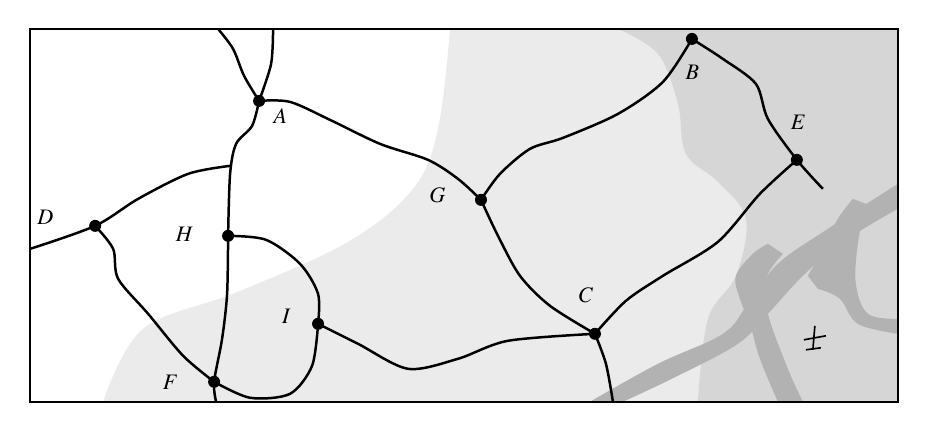
\begin{tikzpicture}[x=0.0127cm,y=-0.0127cm,font=\footnotesize]
\begin{scope}
\clip (12,15) rectangle (880,388);
\fill[black!8] plot[smooth,tension=0.6] coordinates {(85,388) (125,315) (220,278) (330,228) (395,175) (420,115) (432,15)} -- (880,15) -- (880,388) -- cycle;
\fill[black!16] plot[smooth,tension=0.6] coordinates {(600,15) (640,40) (660,90) (668,140) (700,168) (728,205) (718,262) (690,305) (680,388)} -- (880,388) -- (880,15) -- cycle;
\fill[black!30] plot[smooth,tension=0.6] coordinates {(572,388) (640,350) (705,320) (730,290) (760,250) (810,215) (880,170)} -- (880,195) -- plot[smooth,tension=0.6] coordinates {(880,195) (825,228) (785,262) (750,300) (720,330) (660,362) (605,388)} -- cycle;
\fill[black!30] plot[smooth,tension=0.6] coordinates {(760,388) (742,345) (732,310) (722,285) (718,262) (735,240) (750,230)} -- (765,240) -- plot[smooth,tension=0.6] coordinates {(765,240) (748,265) (750,300) (770,355) (785,388)} -- cycle;
\fill[black!30] plot[smooth,tension=0.6] coordinates {(790,262) (805,235) (820,205) (835,185)} -- (848,190) -- plot[smooth,tension=0.6] coordinates {(848,190) (840,230) (838,270) (850,300) (880,305)} -- (880,320) -- plot[smooth,tension=0.6] coordinates {(880,320) (840,310) (822,285) (800,275)} -- cycle;
\end{scope}
\draw (12,15) rectangle (880,388);
\draw (786,326) -- (808,322) (797,312) -- (795,336) (788,336) -- (803,334);
\coordinate (A) at (241,87); \coordinate (B) at (674,25); \coordinate (E) at (779,146);
\coordinate (D) at (77,212); \coordinate (G) at (463,186); \coordinate (H) at (210,222);
\coordinate (C) at (577,320); \coordinate (I) at (300,310); \coordinate (F) at (196,368);
\begin{scope}[line width=0.9pt]
\draw plot[smooth] coordinates {(200,15) (215,35) (226,62) (241,87)};
\draw plot[smooth] coordinates {(255,15) (253,50) (241,87)};
\draw plot[smooth] coordinates {(241,87) (234,112) (218,130) (212,160) (210,222)};
\draw plot[smooth] coordinates {(212,152) (170,160) (120,185) (77,212) (12,235)};
\draw plot[smooth] coordinates {(210,222) (209,280) (204,325) (196,368) (198,388)};
\draw plot[smooth] coordinates {(241,87) (272,88) (312,106) (362,130) (410,146) (440,165) (463,186)};
\draw plot[smooth] coordinates {(463,186) (482,160) (512,135) (545,124) (600,100) (645,68) (674,25)};
\draw plot[smooth] coordinates {(674,25) (705,45) (738,70) (750,105) (779,146) (805,175)};
\draw plot[smooth] coordinates {(463,186) (480,222) (502,262) (532,292) (577,320)};
\draw plot[smooth] coordinates {(577,320) (608,287) (645,262) (700,228) (742,180) (779,146)};
\draw plot[smooth] coordinates {(577,320) (588,350) (595,388)};
\draw plot[smooth] coordinates {(300,310) (340,330) (390,355) (440,345) (490,327) (577,320)};
\draw plot[smooth] coordinates {(77,212) (95,235) (100,265) (130,300) (165,342) (196,368)};
\draw plot[smooth] coordinates {(210,222) (248,226) (282,250) (300,280) (300,310)};
\draw plot[smooth] coordinates {(300,310) (294,352) (272,380) (232,384) (196,368)};
\end{scope}
\foreach \p in {A,B,C,D,E,F,G,H,I} \fill (\p) circle (6);
\node at (262,102) {$A$}; \node at (674,58) {$B$}; \node at (780,108) {$E$}; \node at (27,203) {$D$};
\node at (420,182) {$G$}; \node at (166,220) {$H$}; \node at (568,282) {$C$}; \node at (268,302) {$I$};
\node at (152,368) {$F$};
\end{tikzpicture}
\end{document}